\documentclass{article}
\usepackage[utf8]{inputenc}
\usepackage[spanish]{babel}
\usepackage{listings}
\usepackage{graphicx}
\graphicspath{ {images/} }
\usepackage{cite}

\begin{document}

\begin{titlepage}
    \begin{center}
        \vspace*{1cm}
            
        \Huge
        \textbf{Nociones de la memoria del computador}
            
        \vspace{0.5cm}
        \LARGE
        Informática II
            
        \vspace{1.5cm}
            
        \textbf{Miguel Angel Serna Montoya}
            
        \vfill
            
        \vspace{0.8cm}
            
        \Large
        Departamento de Ingeniería Electrónica y Telecomunicaciones\\
        Universidad de Antioquia\\
        Medellín\\
        Septiembre de 2020
            
    \end{center}
\end{titlepage}

\tableofcontents

\section{Introducción} \label{Introducción}
La idea de este documento es resolver de una vez por todas el verdadero significado de la memoria del computador, ya que es común que muchos de nosotros solo lo relacionemos con el disco duro y la memoria RAM instalada en la placa madre, también, entender como se gestiona, cuales son algunos de sus tipos y definiciones de cada uno.


\section{Contenido} \label{Contenido}

Esta sección es para ver qué pasa con los comandos 
que definen texto

El paquete también agrega un comportamiento especial 
a <<estas marcas para hacer citas textuales>> tal como 
lo indican las reglas de la RAE. \cite{dirac}



A continuación se presenta el logo de C++ Figura (\ref{fig:cpplogo})

\begin{figure}[h]
\includegraphics[width=4cm]{cpplogo.png}
\centering
\caption{Logo de C++}
\label{fig:cpplogo}
\end{figure}
\section{La Memoria del computador}
\subsection{¿Qué es la memoria del computador?}
La memoria es un componente esencial en los computadores, es la herramienta que me permite sacar información del disco duro con alta velocidad de acceso, almacenarla temporalmente y así facilitar el procesamiento de datos e instrucciones que ejecuta la CPU y una vez que estas fueron concretadas regresa la información obtenida a el disco duro reemplazando los archivos que fueron extraídos.
\subsection{Tipos de memoria}
\subsubsection{Memoria ROM:}
Esta memoria se encuentra ubicada en la motherboard, Cuando la computadora se enciende esta se encarga de leer la primera instrucción que hace un chequeo de todos los componentes, posteriormente se carga en esta misma la BIOS que da información sobre los periféricos conectados y sobre que disco duro contiene el sistema operativo. Garantiza que mantendrá los datos que contiene encendida o apagada.
\subsubsection{Memoria Virtual o de SWAMP:}
Esta es la porción de disco duro dedicada exclusivamente a almacenar temporalmente datos de programas y datos de ejecución que se utilizan menos o que ocupan espacio innecesario y así optimizar el almacenamiento de la memoria RAM. Está puede generar problemas al superar su capacidad de almacenamiento.
\subsubsection{Memoria RAM:}
Es aquella memoria a la que accede la CPU para procesar y buscar los datos que se estén usando en el momento y almacenarlos temporalmente y una vez terminada la tarea o cuando pierde su flujo de corriente los datos se pierden.
\subsubsection{Memoria DRAM:}
Es una RAM dinámica de acceso aleatorio que necesita un circuito dinámico de refresco cada cierto tiempo para mantener su funcionalidad, su principal ventaja es el precio y la gran cantidad de posiciones de memoria que puede tener.En la siguiente imagen puede ver una ilustración de una memoria de este estilo. Figura
(\ref{fig:RAMM})
\begin{figure}[h]
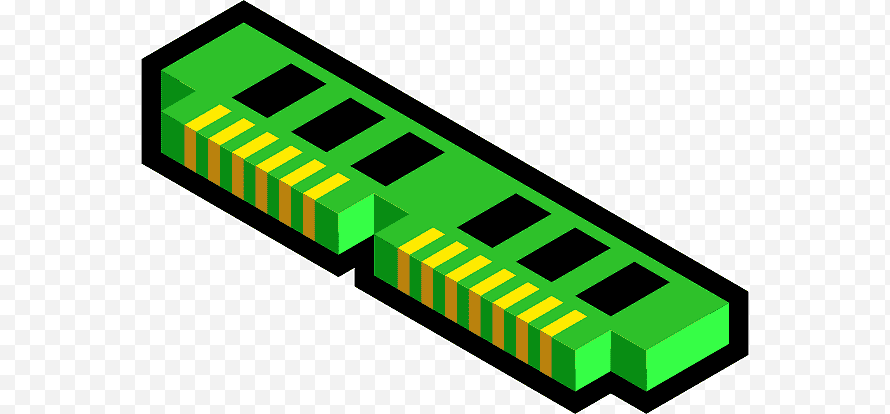
\includegraphics[width=4cm]{RAMM.png}
\centering
\caption{Memoria DRAM}
\label{fig:RAMM}
\end{figure}

\subsubsection{Memoria cache:}
Es una RAM que se caracteriza por ser muy rápida, se empezó a utilizar porque las memorias RAM convencionales ya no eran capaces de acompañar a la velocidad del procesador, haciendo que este se quedara esperando los datos que debía entregar la memoria RAM convencional,no requiere de circuito dinámico de refresco, su desventaja es su precio y capacidad de almacenamiento.
\subsubsection{SRAM:}
Este tipo de memoria RAM basada en semiconductores capaz de mantener la información sin necesidad de circuito de refresco, Un ejemplo de esta es la memoria cache que se encuentra en los microprocesadores.
\subsection{¿Como se gestiona la memoria en un computador?}
Hay un administrador encargado de mantener el control y la forma en que se le asignan espacios en las diferentes memorias, a los procesos y datos. Este gestiona la memoria llevando un registro de las partes de la memoria que se están utilizando y aquellas que no, Asignando espacio en la memoria para los procesos cuando estos los necesitan y Liberando espacio de la memoria asignada a procesos que han terminado. 
\subsection{¿Qué hace que una memoria sea más rápida que otra? ¿Por qué es importante?}
Los factores que influyen en que una memoria

En la sección de teoremas (\ref{Contenido})

\section{Conclusión} \label{Conclusión}
Sin duda alguna, todos los procesos y todo lo que hacemos en la cotidianidad en nuestros computadores seria imposible sin los diferentes tipos de memoria. Gracias a la memoria cache por su gran velocidad que es capaz de sacarle el potencial a nuestro procesador y a la memoria DRAM (en este caso las que se encuentran instaladas en los slots de la placa madre) que tiene una gran capacidad de espacio y es económica, con la ayuda de estas 2 y el disco duro de almacenamiento podemos procesar datos a una gran velocidad.

\bibliographystyle{IEEEtran}
\bibliography{references}

\end{document}
